\documentclass[12pt,a4paper]{book}
\usepackage[utf8]{inputenc}
\usepackage[T1]{fontenc}
\usepackage{hyperref}
\usepackage{amsmath}
\usepackage{amsfonts}
\usepackage[spanish]{babel}
\usepackage{amssymb}
\usepackage{graphicx}
\usepackage[utf8]{inputenc}
\usepackage[left=2.54cm, right=2.54cm, top=2.54cm, bottom=2.54cm]{geometry}
\usepackage{tabularx}
\usepackage{listings}[utf8]
\usepackage{xcolor}
\usepackage{makeidx}
\raggedbottom
\makeindex
\date{\today}

\hypersetup{
	colorlinks=true,
	linkcolor=blue,
	filecolor=magenta,
	urlcolor=cyan,
	pdftitle={Overleaft Example},
}

%Init Python listing configuration
\usepackage{listings}[utf8]
\usepackage{xcolor}

\definecolor{codegreen}{rgb}{0,0.6,0}
\definecolor{codegray}{rgb}{0.5,0.5,0.5}
\definecolor{codepurple}{rgb}{0.58,0,0.82}
\definecolor{backcolour}{rgb}{0.95,0.95,0.92}

\lstdefinestyle{mystyle}{
	backgroundcolor=\color{backcolour},   
	commentstyle=\color{codegreen},
	keywordstyle=\color{blue},
	numberstyle=\tiny\color{codegray},
	stringstyle=\color{codepurple},
	basicstyle=\ttfamily\footnotesize,
	breakatwhitespace=false,         
	breaklines=true,                 
	captionpos=b,
	keepspaces=true,                 
	numbers=left,                    
	numbersep=5pt,                  
	showspaces=false,                
	showstringspaces=false,
	showtabs=false,                  
	tabsize=4,
	classoffset=1,% starting a new class
	morekeywords={True},
	keywordstyle=\color{red},
	classoffset=6,% starting a new class
	morekeywords={True},
	keywordstyle=\color{green},
	classoffset=0,
}


\lstset{
	style=mystyle,
	inputencoding=utf8,
	extendedchars=true,                    
	literate={á}{{\'a}}1 {ã}{{\~a}}1 {é}{{\'e}}1,
}

%Final Python listing configuration

\begin{document}
	\begin{titlepage}
	\noindent
	\centering
	\Large {CONTINUOS INTEGRATION - CONTINUOS DELIVERY}
	\begin{center}
		\centering
		\rule{150 mm}{0.1 mm}
		\Large {DOCKER Y JENKINS\\}
		
		\rule{150 mm}{0.1 mm}
		\large {{SISTEMA DE INTEGRACIÓN CONTINUA Y ENTREGA CONTINUA PARA EL DESARROLLO Y TESTEO DE SOFTWARE}}
		\rule{150 mm}{0.4 mm}
		\vspace{1 cm}
		\vspace{0.3 cm}
		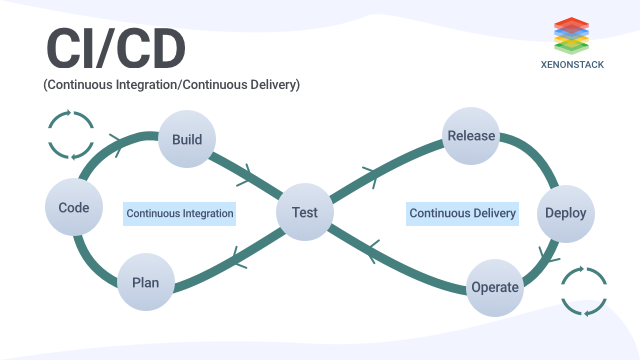
\includegraphics[width=1\textwidth]{image/cover.png}
	\end{center}
	\vspace{0.3 cm}
	\begin{center}
		{\large AUTOR
			{\href{https://github.com/titor-oopart/}{@TITOR-OOPART}}}	\\
		{\large YOUTUBE:	{\href{https://www.youtube.com/@ReadToRun}{@ReadToRun}}}	\\
		{\large GITHUB BOOK:  	{\href{https://github.com/titor-oopart/jenkins_docker_menos_a_mas}{@DOCKER-JENKINS}}}\\
	\end{center}
	\vspace{0.5 cm}
	\vfill
	\begin{center}
		\large\today
	\end{center}
\end{titlepage}
	\tableofcontents
	\chapter{Introducción}
El mayor problea para cualquier proyecto es como lanzar una nueva version de codigo de manera facil y segura, vimos a personas fustrarse trabajando por horas para solucionar problemas de lanzamiento. La idea detras de escribir este libro es simple: hacer los lanzamientos tan facil como sea posible. Este libro apunta a ser la solucion para la implementacion de CI/CD para cada tecnologia enfocandoce en porque el opt para CI y como aplicar en una manera moderna. En otras palabras, queremos que nuestros lectores no necesita nada despues de leer este libro cuando busque ayuda relacionado a cualquier tema CI/CD.
\\
El primer paso hacia estos objetivos. pensamos que seria el flujo, como introducimos el tema y como hacemos la transicion de uno a otro. Este es la rason por que escogemos ir con estilo escrito que es facil seguir: una estilo de narrativa.  Estamos inspirado por "The Phoenix Project" por Gene Kin, Kevin Behr y George Spafford, Leyendo esto es como leer una historia, con su propio giros y vueltas. Al final, tienes no solo que entender la complejidad conceptos pero tambien lee una buena historia. Es facil y apto para que tengamos en mente. Esto es muy diferente de los libros tipicos informativos que no son del agrado de todos. Para estos que no leyeron "Teh Phoenix Project" recomendamos hacerlo\\
Similar, nos gustaria tomar tomar a nuestros lectores en un diario donde el reto mejorara la eficiencia del proyecto por aplicar el principio de CI/CD con la ayuda de docker y jenkins como la tecnologia preferida.
\section{Structure}
En este capitulo discutiremos los siguientes temas:
\begin{itemize}
  \item Introduccion a las caracteristicas
  \item Sprint 1 - Restrospeccion
  \item Luz de esperanza
\end{itemize}
\section{Objetivos}
El objetivo principal de este capitulo es proveer un detallado entendimiento de los conceptos necesarios para el desarrollo de software y como lanzar una nueva version de software puede convertirse en dolor para muchas organizaciones. Seras introducido a muchas caracteristicas, como estan siendo importante en el desarrollo general y recorrido de la aplicacion.
Hay pocos cosas adicionales que aprenderas del capitulo, como el concepto del sprint y el planeamiento del sprint. Este capitulo dadra un idea general de los conceptos y principios de integracion continua.
\section{Introduccion a las caracteristicas}
Un nuevo dia y una maniana fresca. como vi fuer de mi ventana, Vi el mundo moviendose como la semana pasada, sin cambios, no me gustaba. La razon siendo interrumpida; No puedo esperar por una semana larga para finalizar mi web de suspenso en curso serie que me atrapó hasta bien entrada la noche. El problema con ver series que no se detiene el tiempo. Temprano o tarde, eres forsado a irte y preocuparte del siguiente dia. Pero hoy no es muy malo; es un hecho los ultimos dias he estado un poco emocionado como estaba en la mitad del mes en la oficina, un nuevo j
\section{Versionando Database}
Llame a una reunion con el equipo de desarrollo para discurtirlo e introducir al equipo el concepto de database como codigo. Explique como deberiamos llevar los cambios de la base de datos como codigo de la aplicacion. Esto requerira scripting de cada cambio requerido en la bbase de datos y tener lo controlado versionado a travez con el lanzamiento de la aplicacion, "Con el equipo de acuerdo lo agregue" Esto no solo nos ayudara a actualizar la base de datos en un manera manejable, pero esto tambien versionara los cambios el estado de los cambios aplicados. Entonces en caso nosotros necesitemos volver atras a los cambios previos podemos bajar los cambios a la ultima estable.
He listado abajo otros meritos de seguir esta forma
\begin{\begin{itemize}
  \item No hay problemas con la base de datos schema no coincida en multiples ambientes
  \item Incrementa la visibilidad de actualizar la base de datos
  \item Posible configurar una nuevas instancias base de datos desde el script
\end{itemize}}
He explorado como la estructura de base de datos script es generalmente mantenida. Un ejemplo puede ser la siguiente figura
\begin{center}
		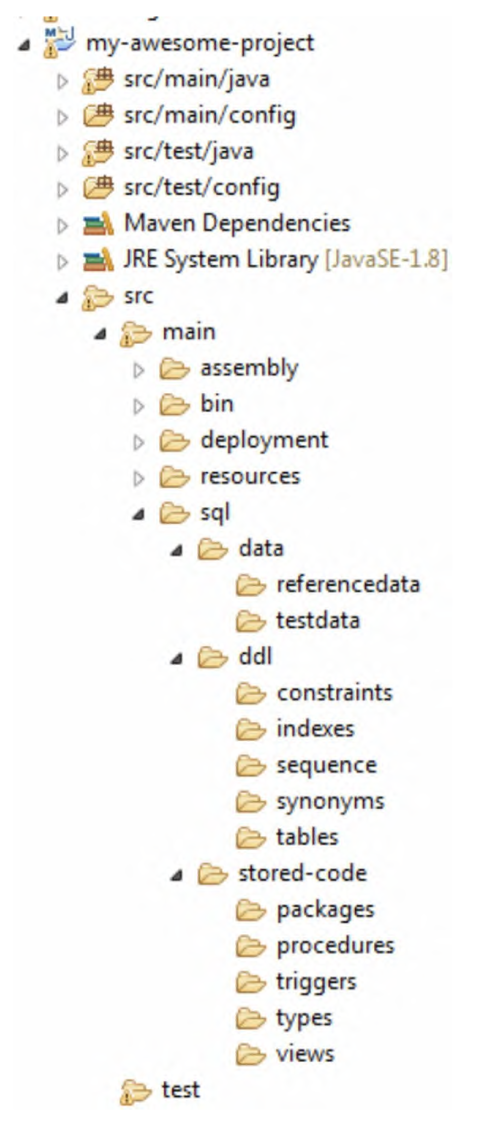
\includegraphics[width=1\textwidth]{image/chapter1/db_structure.png}
\end{center}
\section{Branching strategy}
Que tipo de estrategia es esta?
\begin{center}
		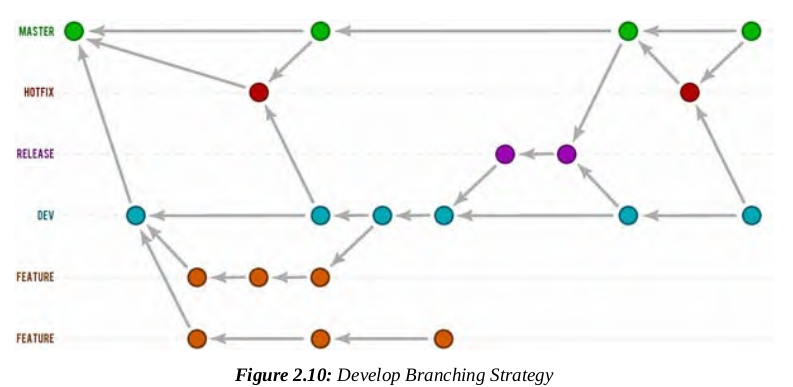
\includegraphics[width=1\textwidth]{image/chapter1/branching.png}
\end{center}
\begin{lstlisting}[language=html]
\end{lstlisting}


\end{document}
